% Shared six-slide body; included by UPDATES.tex.
\begin{frame}{Real-World Scenario: Inspect a Parked Car}
\centering
\begin{tikzpicture}[font=\scriptsize,
 data/.style={-{Stealth},thick,Green}, sight/.style={dashed,thick,Orange}]
\fill[Blue!4,rounded corners](-.8,-.3) rectangle (12.5,4.5);
\fill[Green!9](-.8,-.3)--(12.5,-.3)--(12.5,.7)--(9.2,1.1)--(5.5,.5)--(2.1,1)--(-.8,.6)--cycle;
% Car silhouette: wheels, body, cabin, windows and headlights.
\foreach \x in {4.85,6.05}{\filldraw[draw=Navy,fill=gray!70](\x,.96) circle (.22);\fill[gray!20](\x,.96) circle (.10);}
\filldraw[draw=Navy,fill=Blue!25,rounded corners=3pt](4.35,1.02)--(4.35,1.35)--(4.83,1.48)--(5.13,1.99)--(5.95,1.99)--(6.3,1.5)--(6.65,1.38)--(6.65,1.02)--cycle;
\filldraw[draw=Navy,fill=white](4.99,1.53)--(5.23,1.87)--(5.52,1.87)--(5.52,1.53)--cycle;
\filldraw[draw=Navy,fill=white](5.61,1.53)--(5.61,1.87)--(5.88,1.87)--(6.12,1.53)--cycle;
\draw[Navy](5.56,1.45)--(5.56,1.08);
\draw[Navy,thick](5.35,1.38)--(5.46,1.38);
\fill[Orange!70](6.42,1.23) rectangle (6.62,1.34);
\node[below,align=center] at (5.6,.67) {Parked car: known GPS region};
\foreach \x/\y/\name in {1.5/3.5/A: rear-side view,5.65/3.9/B: roof view,9/3.3/C: front-side view}{
 \begin{scope}[shift={(\x,\y)}]
 \draw[Navy,thick](-.38,-.16)--(.38,.16) (-.38,.16)--(.38,-.16);
 \foreach \a in {-.38,.38}\foreach \b in {-.16,.16}{\draw[Navy,fill=Blue!10](\a,\b) ellipse (.19 and .07);}
 \fill[Blue](-.13,-.12) rectangle (.13,.12);
 \draw[Navy,thick](0,-.12)--(0,-.3);
 \draw[Navy,fill=Orange!20](-.1,-.30) rectangle (.1,-.45);
 \fill[Navy](0,-.38) circle (.035);
 \node[above,font=\scriptsize\bfseries,text=Navy] at (0,.3){UAV \name};
 \end{scope}}
\fill[Orange,opacity=.12](1.5,3.05)--(4.5,1.2)--(5.4,2)--cycle;
\fill[Orange,opacity=.12](5.65,3.45)--(5.05,2.05)--(6.65,2.05)--cycle;
\fill[Orange,opacity=.12](9,2.85)--(6.1,.95)--(6.65,2.05)--cycle;
\draw[sight](1.5,3.05)--(4.8,1.7);\draw[sight](5.65,3.45)--(5.65,2);\draw[sight](9,2.85)--(6.4,1.55);
\node[draw=Navy,fill=white,rounded corners,align=center,minimum height=.65cm](gs) at (1.2,.3){Ground station\\Map + annotated views};
\node[draw=Green,fill=white,rounded corners,align=center,minimum height=.65cm](gpu) at (10.7,1.25){Selected GPU UAV\\Analyze + combine};
\draw[data](1.95,3.6) to[bend left=15](gpu.north);
\draw[data](6.15,3.9) to[bend left=10](gpu.north);
\draw[data](9.45,3.3)--(gpu.north);
\draw[data](gpu.south)--(10.7,-.05)--(1.2,-.05)--(gs.south);
\node[fill=white,text=Green] at (8.6,4.28){Named image Data};
\node[fill=white,text=Green] at (9.5,.12){Results + image access};
\node[align=left,text=Navy] at (1.4,1.8){Each camera UAV needs:\\GPS/IMU pose\\Gimbal + camera API};
\end{tikzpicture}
\evidence{Illustrative field scenario, not a completed flight experiment. Orange: camera view. Green: application data flow, not flight paths.}
\end{frame}

\begin{frame}{NDNSF Connects Roles; Sensors Must Deliver the Views}
\centering
\begin{tikzpicture}[node distance=.25cm,font=\small,
 b/.style={draw=Navy,rounded corners,fill=Blue!6,text width=2.1cm,minimum height=1.1cm,align=center}]
\node[b](r){Request\\Car location + constraints};
\node[b,right=of r](o){ACK\\Camera / GPU offers};
\node[b,right=of o](s){Selection\\Views + Analyzer};
\node[b,right=of s](v){Execute\\Capture + analyze};
\node[b,right=of v](e){Response\\Annotations + image access};
\foreach \a/\b in {r/o,o/s,s/v,v/e}{\draw[-{Stealth},thick,Navy](\a)--(\b);}
\end{tikzpicture}
\vspace{.8em}
\begin{itemize}
\item \textbf{NDNSF}: discover authorized Providers, assign roles, retrieve protected data and track completion.
\item \textbf{UAV application}: navigate, point the camera, capture and validate the observation.
\item \textbf{Perception}: detect the car, associate the same car across views and combine evidence.
\end{itemize}
\claim{Successful message exchange does not prove that a UAV captured the right target.}
\evidence{Proposed inspection workflow; component/simulation evidence does not establish field qualification.}
\end{frame}

\begin{frame}{Three Gaps Between Simulation and the Field}
\small\renewcommand{\arraystretch}{1.5}
\begin{tabular}{>{\RaggedRight\arraybackslash}p{.20\textwidth}>{\RaggedRight\arraybackslash}p{.28\textwidth}>{\RaggedRight\arraybackslash}p{.42\textwidth}}
\textbf{Gap}&\textbf{Simplified example}&\textbf{Real deployment needs}\\\hline
Position / pointing & Known coordinates; assigned views & GPS + IMU, camera/gimbal calibration, coordinate frames, synchronized pose and exposure\\
Useful images & Car assumed visible & Real control/capture APIs, feedback, blur/occlusion checks and bounded retries\\
Multi-view analysis & Images supplied to a detector & Same-target association, uncertainty-aware fusion and independent ground truth\\
\end{tabular}
\claim{Known GPS narrows the search; it does not guarantee visibility or make three detections a reliable multi-view result.}
\evidence{Candidate tools: \href{https://mavsdk.mavlink.io/main/en/cpp/index.html}{MAVSDK control/telemetry}; \href{https://docs.opencv.org/4.13.0/d9/d0c/group__calib3d.html}{OpenCV calibration/geometry}. Hardware support and integration remain to be verified.}
\end{frame}

\begin{frame}{Close One Physical Loop Before Adding More UAVs}
\centering
\begin{tikzpicture}[font=\small,
 b/.style={draw=Navy,rounded corners,fill=Blue!6,text width=2.45cm,minimum height=1.1cm,align=center}]
\node[b](p) at (0,0){Locate + plan\\Car location and aircraft pose};
\node[b](m) at (3.3,0){Move + point\\Observe arrival and gimbal angle};
\node[b](c) at (6.6,0){Capture + check\\Frame, timestamp, visibility};
\node[b,draw=Green,fill=Green!7](o) at (9.9,0){Publish + analyze\\Verified view + metadata};
\foreach \a/\b in {p/m,m/c,c/o}{\draw[-{Stealth},thick,Navy](\a)--(\b);}
\draw[-{Stealth},thick,Orange](c.south)--++(0,-.8)-| node[pos=.25,below,font=\scriptsize]{Bad view: bounded retry or explicit failure}(m.south);
\end{tikzpicture}
\vspace{1.5em}
\begin{itemize}
\item A control ACK is not capture success: check the image and measured camera pose.
\item A pixel needs geometry/depth for world localization; views need correspondence before fusion.
\item Keep stabilization and safety rejection onboard, independent of network delays.
\end{itemize}
\evidence{Proposed feedback loop: reject stale pose, missing frames and exhausted deadlines.}
\end{frame}

\begin{frame}{A Short Route to a Credible Field Demonstration}
\small
\begin{enumerate}
\item \textbf{Bench}: one real camera/gimbal; verify commands, capture, calibration and pose/time alignment.
\item \textbf{Flight simulation}: use the same adapter; inject navigation error, occlusion and link loss. Use \href{https://docs.px4.io/main/en/simulation/}{PX4 software/hardware-in-the-loop} where supported.
\item \textbf{One UAV}: inspect a parked car at a surveyed location; measure pointing error, useful-view rate and latency.
\item \textbf{Multiple UAVs}: compare one versus complementary views; measure recognition quality, time/energy cost and participant failures.
\end{enumerate}
\claim{Next milestone: one real, correctly aimed image with synchronized pose and independently checked target visibility.}
\evidence{Planned stages, not completed experiments. Start with a parked car; moving-car tracking is outside this first demonstration.}
\end{frame}

\begin{frame}{Available Hardware: Programmable Gimbal Cameras}
\fontsize{9}{10.5}\selectfont
\begin{columns}[T,onlytextwidth]
\column{.48\textwidth}
\centering\textbf{\large\color{Navy}SIYI A8 mini}\par
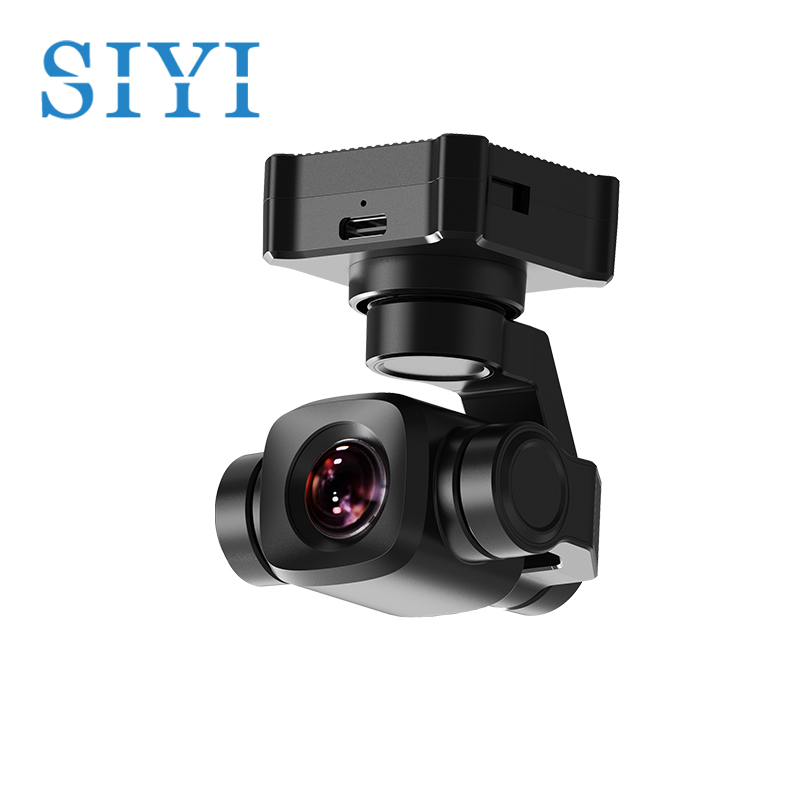
\includegraphics[height=2.8cm,width=.8\linewidth,keepaspectratio]{assets/siyi-a8-mini-official.jpg}\par
\raggedright
\begin{itemize}
\item Camera + three-axis gimbal in one unit.
\item Ethernet UDP / UART control; Ethernet video.
\end{itemize}
\column{.48\textwidth}
\centering\textbf{\large\color{Navy}Gremsy Pixy U}\par
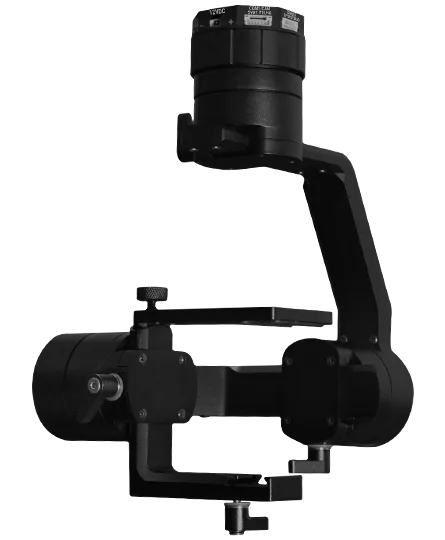
\includegraphics[height=2.8cm,width=.8\linewidth,keepaspectratio]{assets/gremsy-pixy-u-official.png}\par
\raggedright
\begin{itemize}
\item Gimbal only; add a compatible camera.
\item SDK / MAVLink control; verify camera support.
\end{itemize}
\end{columns}
\vspace{.6em}
\textbf{First bench test:} command an angle $\rightarrow$ read actual attitude $\rightarrow$ capture the parked car.
\evidence{Product images: \href{https://shop.siyi.biz/products/siyi-a8-mini-gimbal-camera}{SIYI official store} and \href{https://gremsy.com/products/pixy-u}{Gremsy official site}. Images not to scale. Candidate hardware; verify power, payload and mounting before selection.}
\end{frame}
